\documentclass[hyperref={unicode}]{beamer}

\usepackage[IL2]{fontenc}
\usepackage[utf8]{inputenc}
\usepackage[czech]{babel}
\usepackage{graphicx}
\usepackage{float}
\usepackage{listings}
\usetheme{Madrid}

\title[ITY 5. projekt]{Prohledávání do šířky}
\subtitle{Grafové algoritmy}
\author{Alexandr Chalupnik}
\date{\today}

\begin{document}

%uvodni strana 
\frame{\titlepage}

%obsah
\begin{frame}
\frametitle{Obsah}
\tableofcontents
\end{frame}

\section{Definice}
\begin{frame}
\frametitle{Co je to graf}
\begin{block}{Neformální definice}
Grafy si můžeme představit jako zjednodušení reálného světa, kde studovaný problém znázorníme pomocí bodů a čar, které je spojují, a tím popisují vlastnosti. Takovým bodům pak v teorii grafů říkáme vrcholy grafu a čáry, které je spojují, nazýváme hrany grafu.\cite{definice:neformalni}
\end{block}
\begin{block}{Formální definice}
Graf \alert{je dvojice} $G = (V,E)$, kde $V$ je množina vrcholů (vertex) a $E$ je množina hran (edge).
\end{block}
\end{frame}

\section{Popis algoritmu}
\begin{frame}[fragile]
\frametitle{Pseudokód}
\begin{lstlisting}[basicstyle=\footnotesize\ttfamily,breaklines=true]
BFS(s){
    Q = Queue()
    V = List()
    Q.enqueue(s)
    
    while (Q is not empty){
        v  =  Q.dequeue()
        V.push(v)
        for(all neighbours w of v){
            if (w not in V){ 
                Q.enqueue(w)
            }
        }
    }
}
\end{lstlisting}
\scriptsize{inspirování z: \cite{pseudo}}
\end{frame}

\begin{frame}{Slovní popis}
\begin{enumerate}
  \setbeamertemplate{enumerate items}[default]
    \item vytvoř frontu Q a seznam navštívených vrcholů V
    \item přidej počáteční vrchol s do fronty Q
    \item pokud není fronta Q prázdná vyjmi vrchol z fronty Q a vlož ho do seznamu navštívených vrcholů, jinak ukonči procházení
    \item přidej každý dětský vrchol, který nebyl ještě nebyla navštívený do fronty Q
    \item pokračuj krokem 3
\end{enumerate}
\end{frame}

\section{Ukázka}
\begin{frame}
\begin{block}{Postup}
\begin{enumerate}
  \setbeamertemplate{enumerate items}[default]
    \item vytvoř frontu Q a seznam navštívených vrcholů V
    \item přidej počáteční vrchol s do fronty Q
\end{enumerate}
\end{block}
  \begin{columns}[T]
    \begin{column}{0.3\linewidth}
        \begin{figure}
        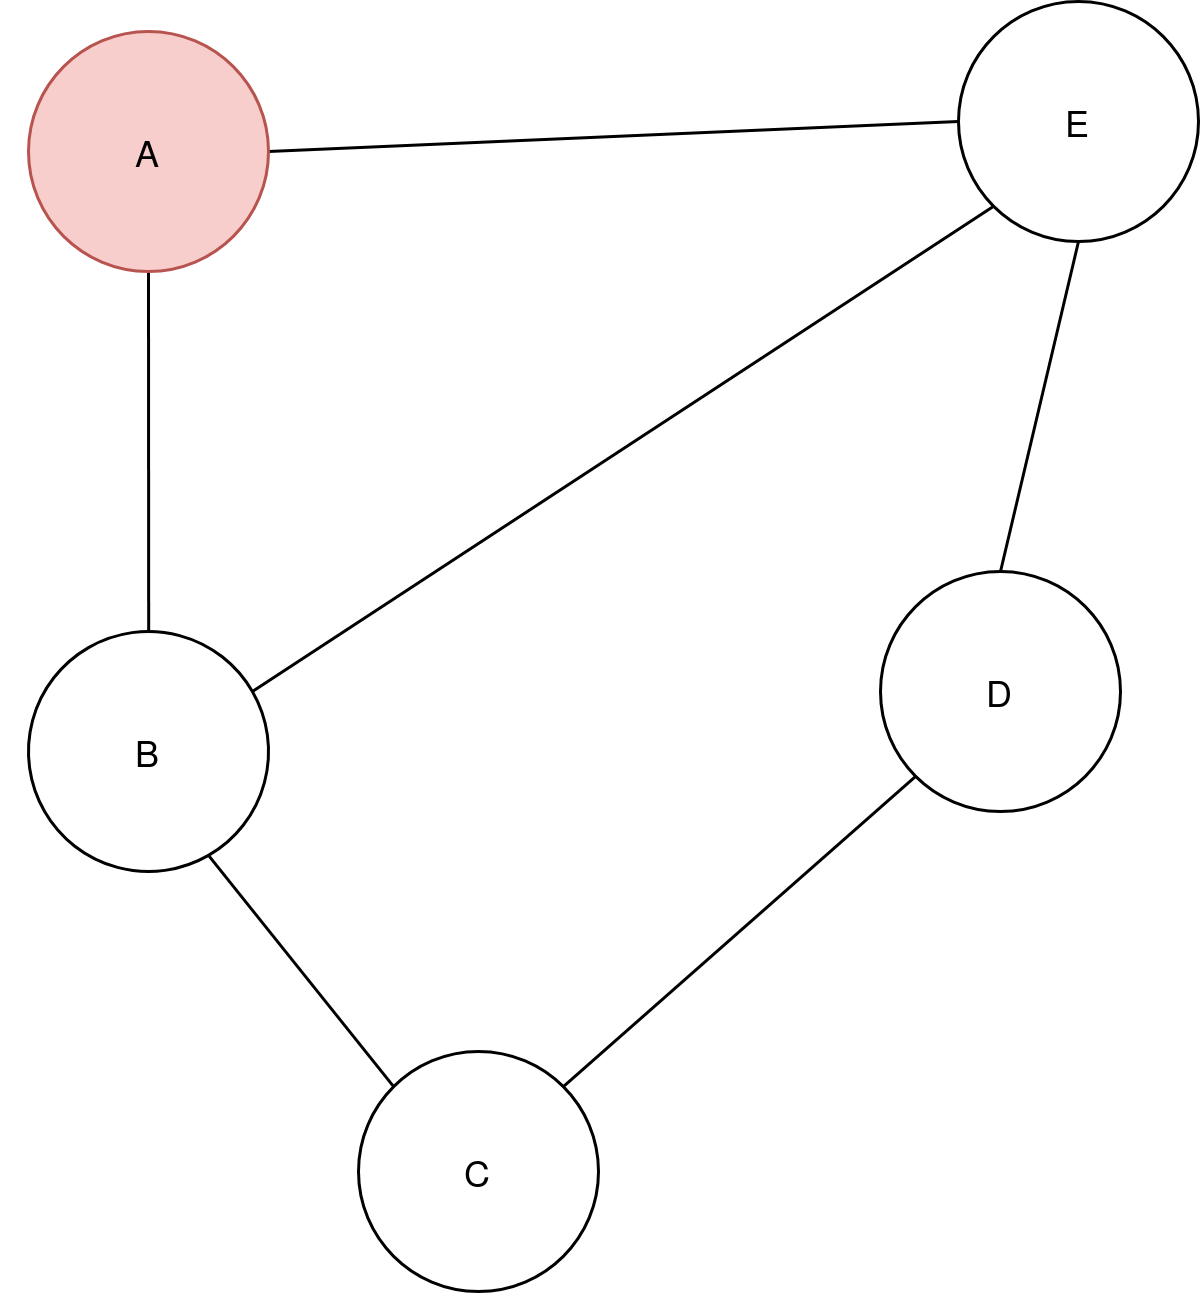
\includegraphics[width=\linewidth]{state1.png}
        \end{figure}
    \end{column}
    \begin{column}{0.3\linewidth}
    \begin{table}[]
        \begin{tabular}{|l||l|l|l|}
        \hline
        Q & A &  &  \\ \hline
        V &  &  &  \\ \hline
        \end{tabular}
\end{table}
    \end{column}
  \end{columns}
\end{frame}

\begin{frame}
\begin{block}{Postup}
\begin{enumerate}
  \setbeamertemplate{enumerate items}[default]
    \item pokud není fronta Q prázdná vyjmi vrchol z fronty Q a vlož ho do seznamu navštívených vrcholů, jinak ukonči procházení
    \item přidej každý dětský vrchol, který nebyl ještě nebyla navštívený do fronty Q
\end{enumerate}
\end{block}
  \begin{columns}[T]
    \begin{column}{0.3\linewidth}
        \begin{figure}
        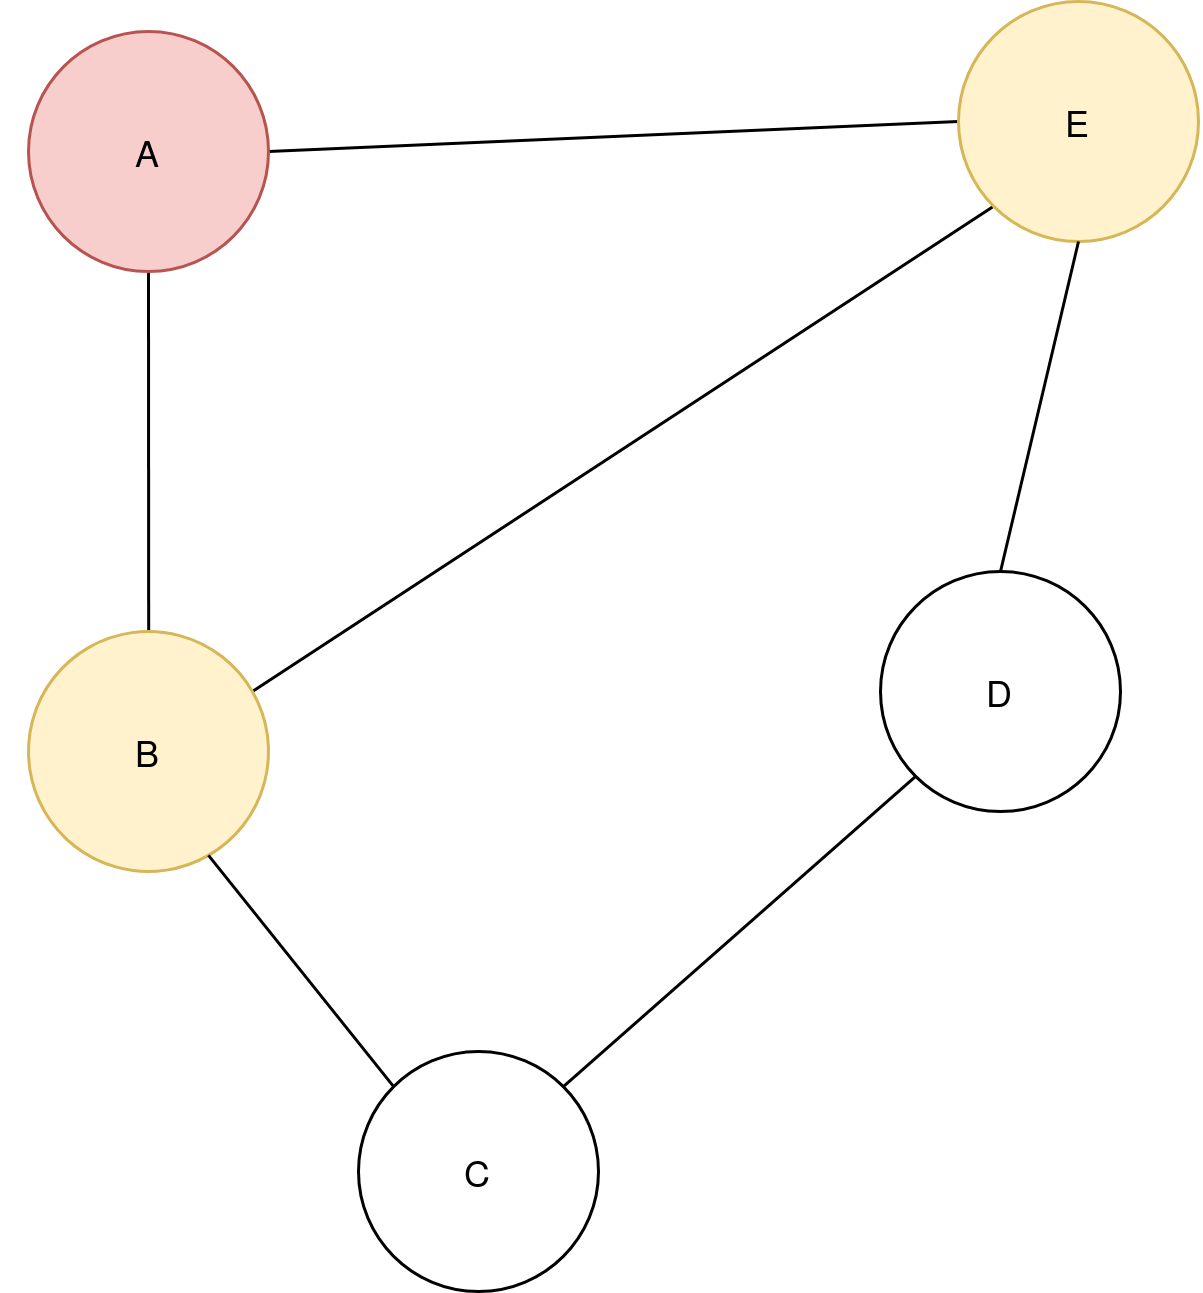
\includegraphics[width=\linewidth]{state2.png}
        \end{figure}
    \end{column}
    \begin{column}{0.3\linewidth}
    \begin{table}[]
        \begin{tabular}{|l||l|l|l|}
        \hline
        Q & B & E &  \\ \hline
        V & A &  &  \\ \hline
        \end{tabular}
\end{table}
    \end{column}
  \end{columns}
\end{frame}

\begin{frame}
\begin{block}{Postup}
\begin{enumerate}
  \setbeamertemplate{enumerate items}[default]
    \item pokud není fronta Q prázdná vyjmi vrchol z fronty Q a vlož ho do seznamu navštívených vrcholů, jinak ukonči procházení
\end{enumerate}
\end{block}
  \begin{columns}[T]
    \begin{column}{0.3\linewidth}
        \begin{figure}
        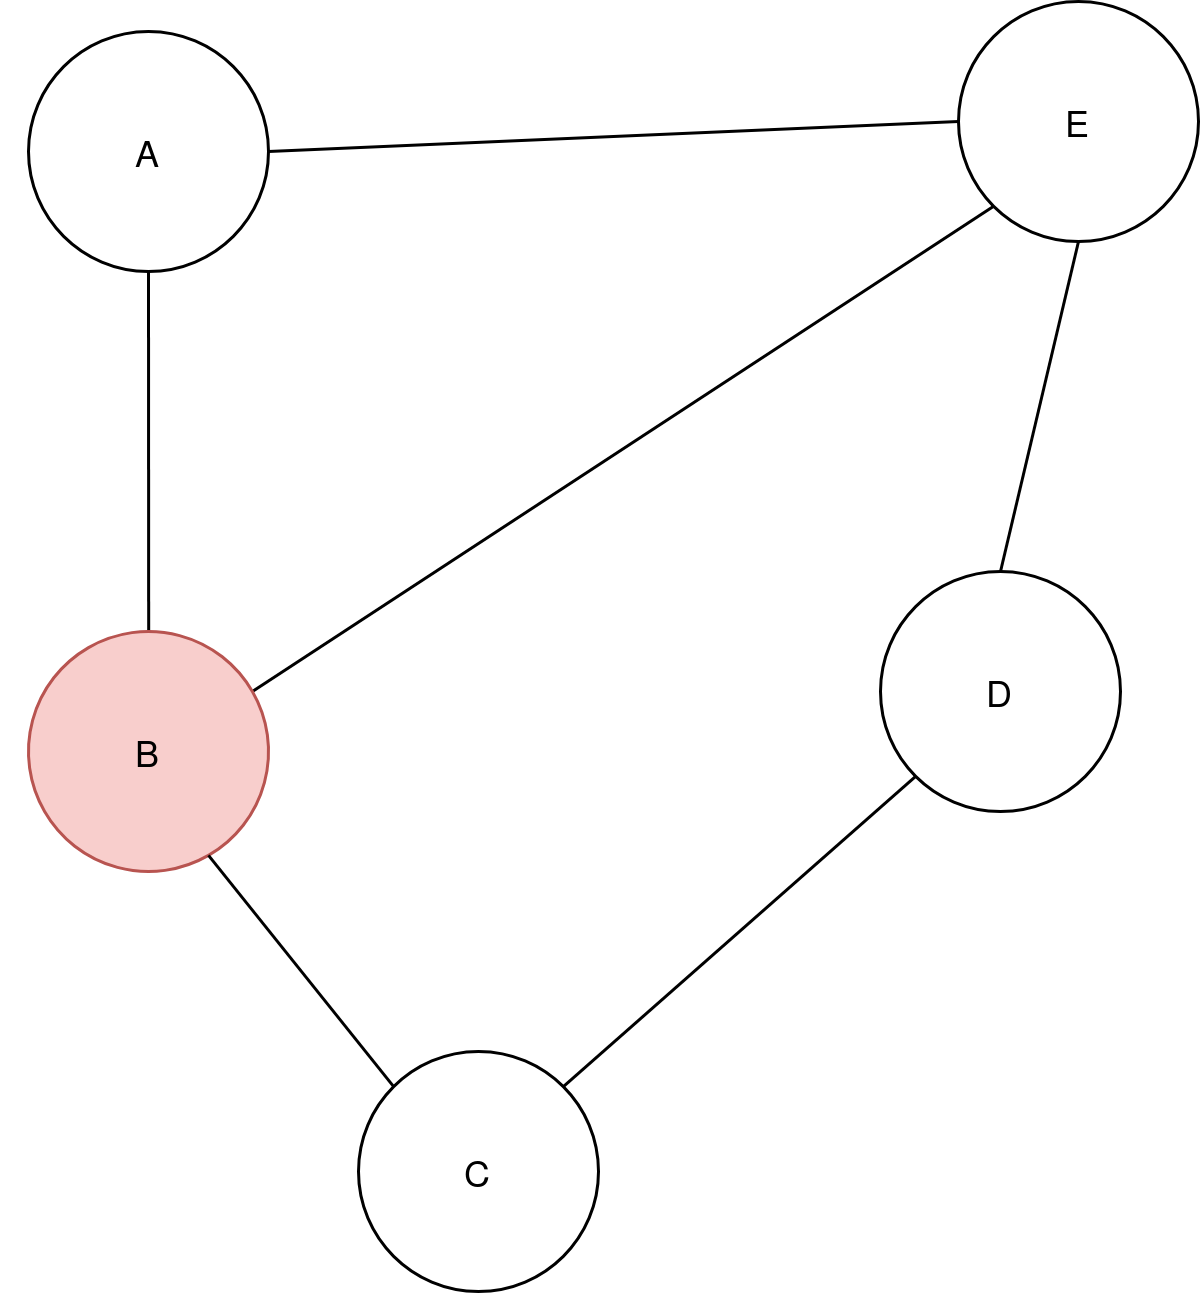
\includegraphics[width=\linewidth]{state3.png}
        \end{figure}
    \end{column}
    \begin{column}{0.3\linewidth}
    \begin{table}[]
        \begin{tabular}{|l||l|l|l|}
        \hline
        Q & E &  &  \\ \hline
        V & A & B &  \\ \hline
        \end{tabular}
\end{table}
    \end{column}
  \end{columns}
\end{frame}

\begin{frame}
\begin{block}{Postup}
\begin{enumerate}
  \setbeamertemplate{enumerate items}[default]
    \item přidej každý dětský vrchol, který nebyl ještě nebyla navštívený do fronty Q
\end{enumerate}
\end{block}
  \begin{columns}[T]
    \begin{column}{0.3\linewidth}
        \begin{figure}
        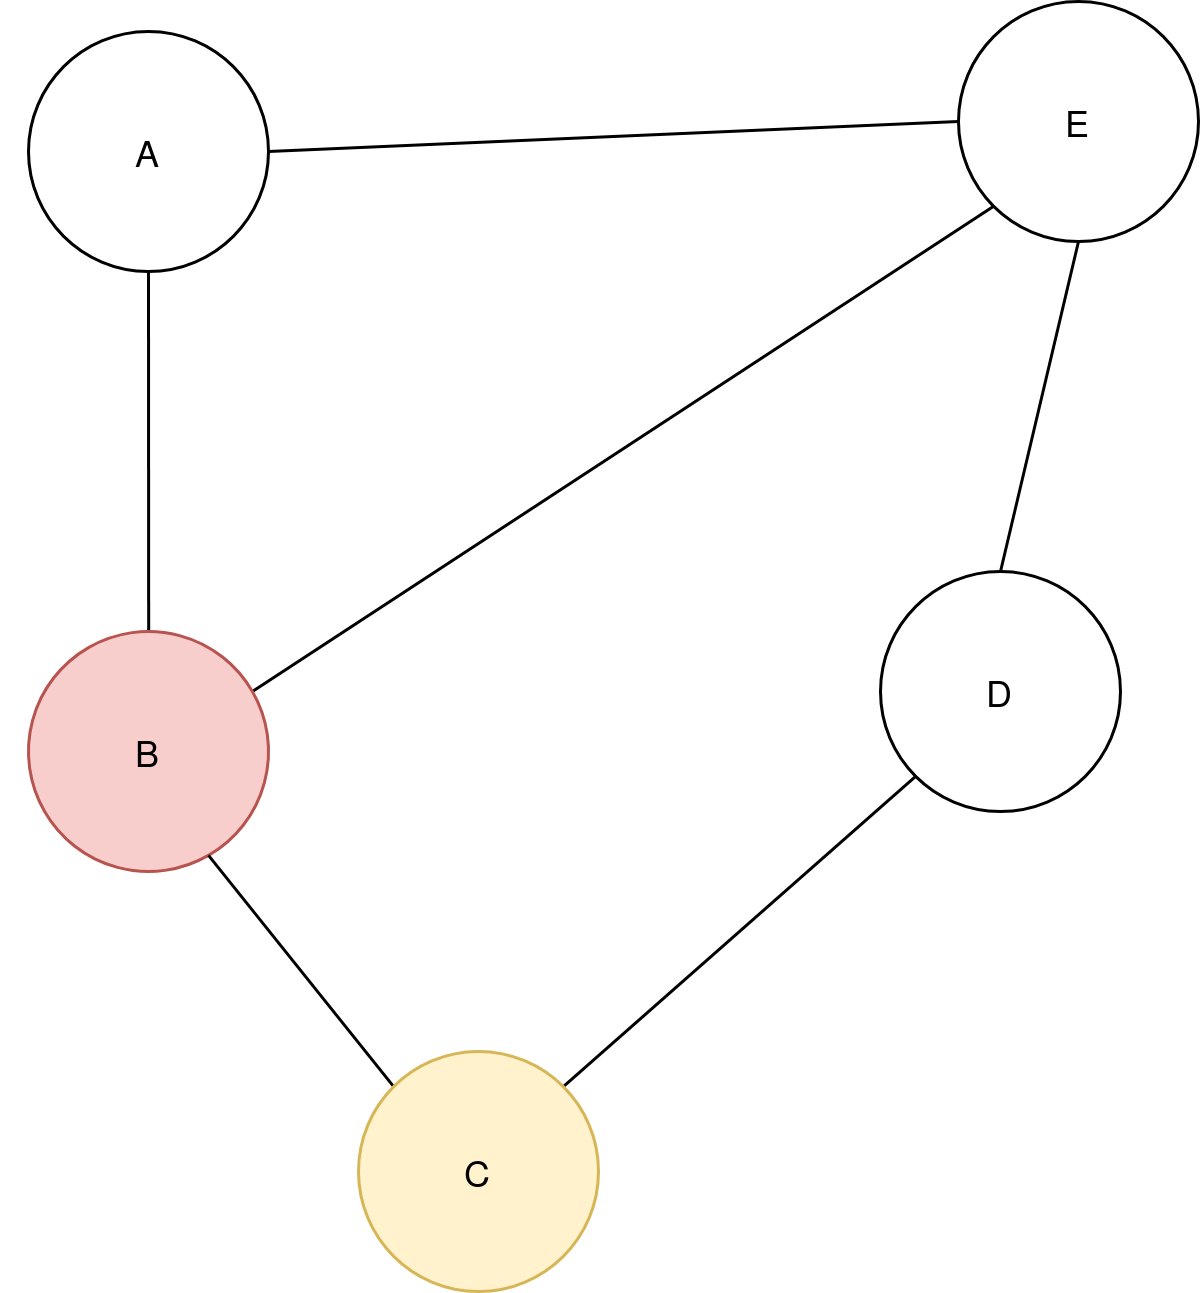
\includegraphics[width=\linewidth]{state4.png}
        \end{figure}
    \end{column}
    \begin{column}{0.3\linewidth}
    \begin{table}[]
        \begin{tabular}{|l||l|l|l|}
        \hline
        Q & E & C &  \\ \hline
        V & A & B &  \\ \hline
        \end{tabular}
\end{table}
    \end{column}
  \end{columns}
\end{frame}

\begin{frame}
\begin{block}{Postup}
\begin{enumerate}
  \setbeamertemplate{enumerate items}[default]
    \item pokud není fronta Q prázdná vyjmi vrchol z fronty Q a vlož ho do seznamu navštívených vrcholů, jinak ukonči procházení
\end{enumerate}
\end{block}
  \begin{columns}[T]
    \begin{column}{0.3\linewidth}
        \begin{figure}
        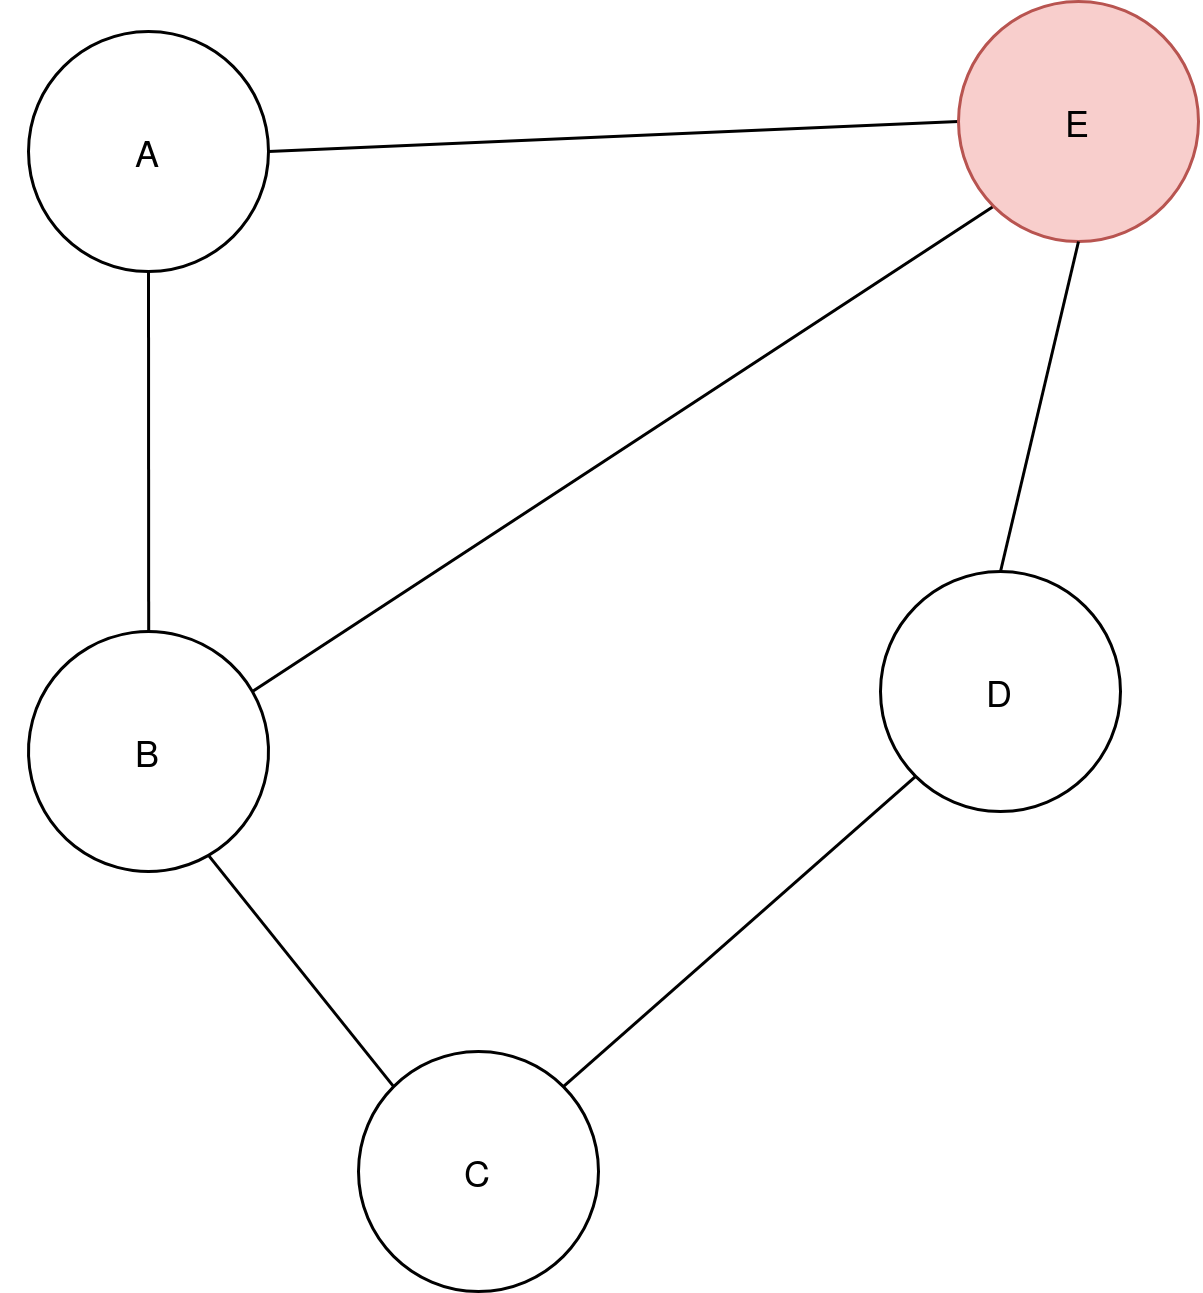
\includegraphics[width=\linewidth]{state5.png}
        \end{figure}
    \end{column}
    \begin{column}{0.3\linewidth}
    \begin{table}[]
        \begin{tabular}{|l||l|l|l|}
        \hline
        Q & C &  &  \\ \hline
        V & A & B & E  \\ \hline
        \end{tabular}
\end{table}
    \end{column}
  \end{columns}
\end{frame}

\begin{frame}
\begin{block}{Postup}
\begin{enumerate}
  \setbeamertemplate{enumerate items}[default]
    \item přidej každý dětský vrchol, který nebyl ještě nebyla navštívený do fronty Q
\end{enumerate}
\end{block}
  \begin{columns}[T]
    \begin{column}{0.3\linewidth}
        \begin{figure}
        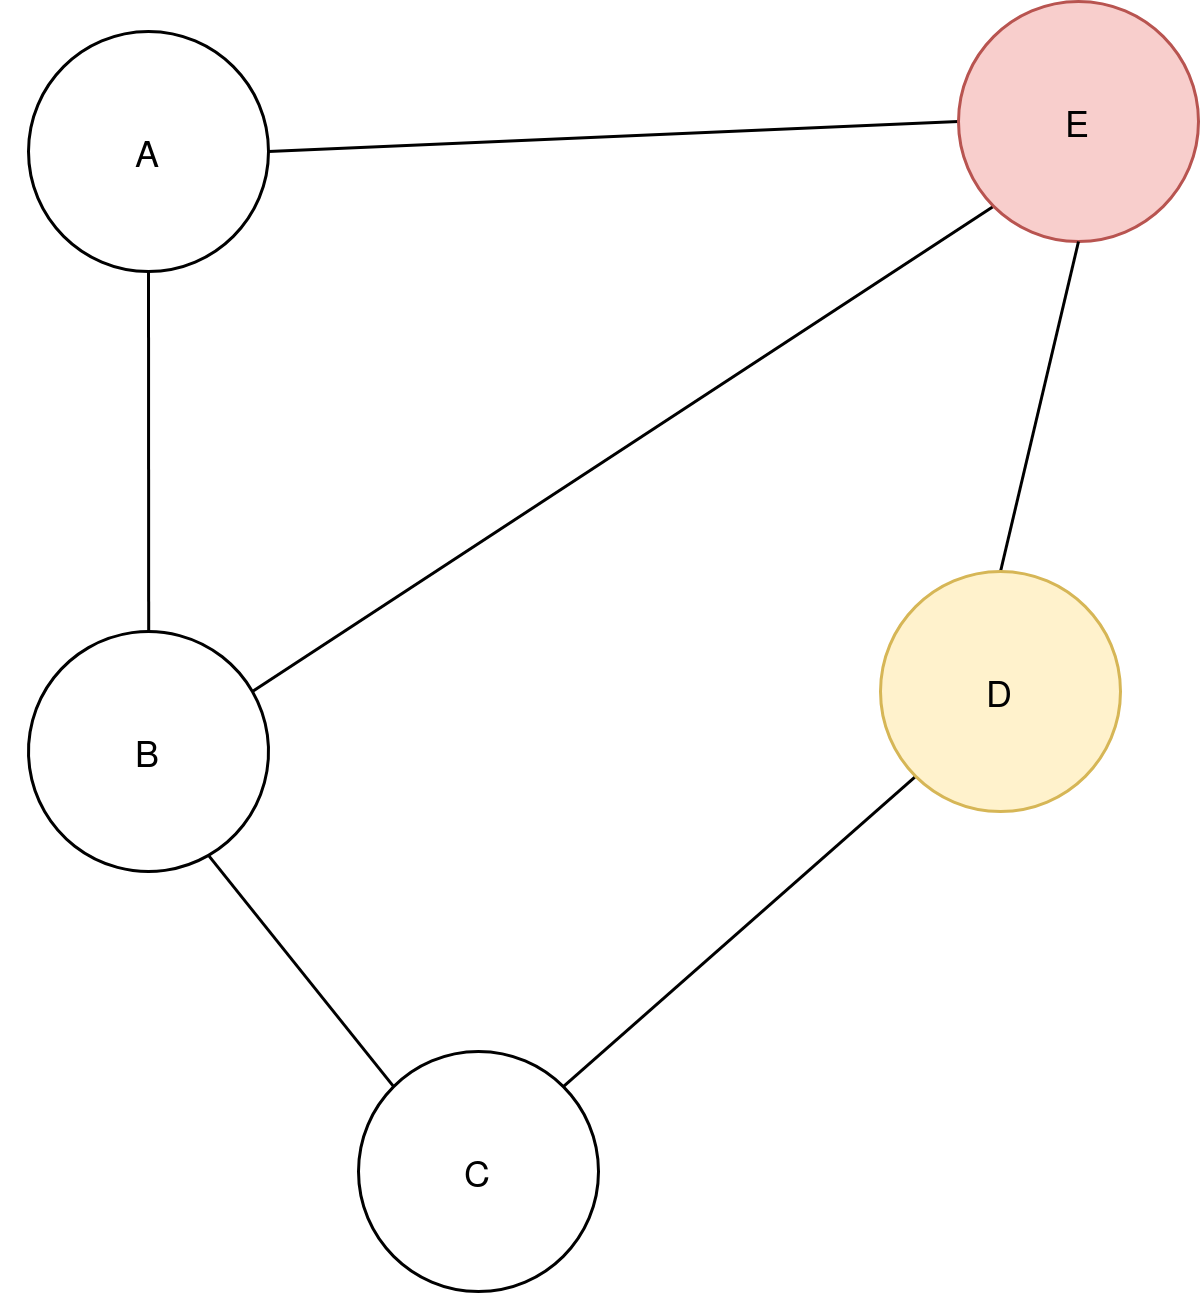
\includegraphics[width=\linewidth]{state6.png}
        \end{figure}
    \end{column}
    \begin{column}{0.3\linewidth}
    \begin{table}[]
        \begin{tabular}{|l||l|l|l|}
        \hline
        Q & C & D &  \\ \hline
        V & A & B & E  \\ \hline
        \end{tabular}
\end{table}
    \end{column}
  \end{columns}
\end{frame}

\begin{frame}
\begin{block}{Postup}
\begin{enumerate}
  \setbeamertemplate{enumerate items}[default]
    \item pokud není fronta Q prázdná vyjmi vrchol z fronty Q a vlož ho do seznamu navštívených vrcholů, jinak ukonči procházení
\end{enumerate}
\end{block}
  \begin{columns}[T]
    \begin{column}{0.3\linewidth}
        \begin{figure}
        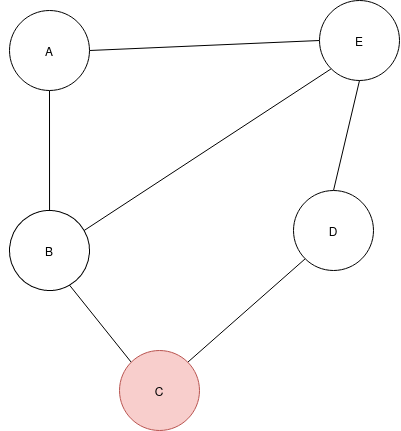
\includegraphics[width=\linewidth]{state7.png}
        \end{figure}
    \end{column}
    \begin{column}{0.3\linewidth}
    \begin{table}[]
        \begin{tabular}{|l||l|l|l|l|}
        \hline
        Q & D &   &   &   \\ \hline
        V & A & B & E & C \\ \hline
        \end{tabular}
\end{table}
    \end{column}
  \end{columns}
\end{frame}

\begin{frame}
\begin{block}{Postup}
\begin{enumerate}
  \setbeamertemplate{enumerate items}[default]
    \item pokud není fronta Q prázdná vyjmi vrchol z fronty Q a vlož ho do seznamu navštívených vrcholů, jinak ukonči procházení
\end{enumerate}
\end{block}
  \begin{columns}[T]
    \begin{column}{0.3\linewidth}
        \begin{figure}
        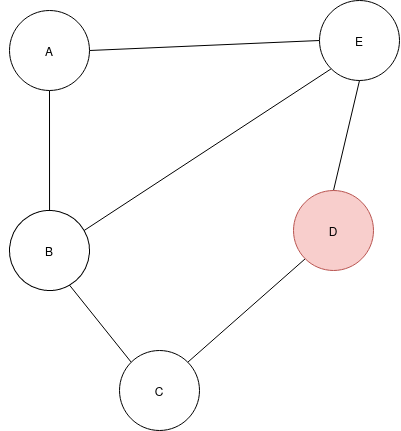
\includegraphics[width=\linewidth]{state8.png}
        \end{figure}
    \end{column}
    \begin{column}{0.4\linewidth}
    \begin{table}[]
        \begin{tabular}{|l||l|l|l|l|l|}
        \hline
        Q &   &   &   &   &   \\ \hline
        V & A & B & E & C & D \\ \hline
        \end{tabular}
\end{table}
    \end{column}
  \end{columns}
\end{frame}

\begin{frame}
\begin{block}{Postup}
Asymptotická časová složitost algoritmu je $O(|V| + |E|)$, kde $|V|$ je počet vrcholů a $|E|$ je počet hran grafu\cite{complex}.
\end{block}
  \begin{columns}[T]
    \begin{column}{0.3\linewidth}
        \begin{figure}
        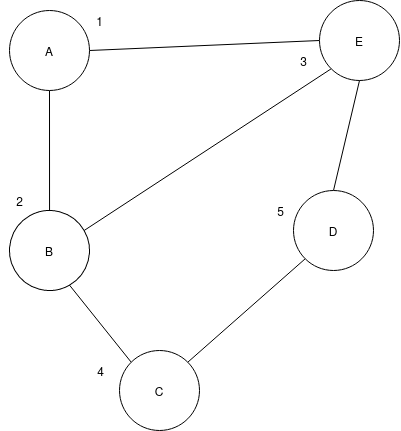
\includegraphics[width=\linewidth]{final_state.png}
        \end{figure}
    \end{column}
    \begin{column}{0.4\linewidth}
    \begin{table}[]
        \begin{tabular}{|l||l|l|l|l|l|}
        \hline
        V & A & B & E & C & D \\ \hline
        \end{tabular}
\end{table}
    \end{column}
  \end{columns}
\end{frame}






%http://texnorte.blogspot.com/2013/10/beamer-bibliography-icon.html
%https://www.overleaf.com/learn/latex/bibliography_management_with_bibtex
\section{Bibliografie}
\begin{frame}
\frametitle{Literatura}
\setbeamertemplate{bibliography item}[text]
\bibliographystyle{czechiso}
\bibliography{proj5}
\end{frame}

\end{document}

